% Options for packages loaded elsewhere
\PassOptionsToPackage{unicode}{hyperref}
\PassOptionsToPackage{hyphens}{url}
%
\documentclass[
]{book}
\usepackage{lmodern}
\usepackage{amssymb,amsmath}
\usepackage{ifxetex,ifluatex}
\ifnum 0\ifxetex 1\fi\ifluatex 1\fi=0 % if pdftex
  \usepackage[T1]{fontenc}
  \usepackage[utf8]{inputenc}
  \usepackage{textcomp} % provide euro and other symbols
\else % if luatex or xetex
  \usepackage{unicode-math}
  \defaultfontfeatures{Scale=MatchLowercase}
  \defaultfontfeatures[\rmfamily]{Ligatures=TeX,Scale=1}
\fi
% Use upquote if available, for straight quotes in verbatim environments
\IfFileExists{upquote.sty}{\usepackage{upquote}}{}
\IfFileExists{microtype.sty}{% use microtype if available
  \usepackage[]{microtype}
  \UseMicrotypeSet[protrusion]{basicmath} % disable protrusion for tt fonts
}{}
\makeatletter
\@ifundefined{KOMAClassName}{% if non-KOMA class
  \IfFileExists{parskip.sty}{%
    \usepackage{parskip}
  }{% else
    \setlength{\parindent}{0pt}
    \setlength{\parskip}{6pt plus 2pt minus 1pt}}
}{% if KOMA class
  \KOMAoptions{parskip=half}}
\makeatother
\usepackage{xcolor}
\IfFileExists{xurl.sty}{\usepackage{xurl}}{} % add URL line breaks if available
\IfFileExists{bookmark.sty}{\usepackage{bookmark}}{\usepackage{hyperref}}
\hypersetup{
  pdftitle={A Minimal Book Example},
  pdfauthor={Yihui Xie},
  hidelinks,
  pdfcreator={LaTeX via pandoc}}
\urlstyle{same} % disable monospaced font for URLs
\usepackage{color}
\usepackage{fancyvrb}
\newcommand{\VerbBar}{|}
\newcommand{\VERB}{\Verb[commandchars=\\\{\}]}
\DefineVerbatimEnvironment{Highlighting}{Verbatim}{commandchars=\\\{\}}
% Add ',fontsize=\small' for more characters per line
\usepackage{framed}
\definecolor{shadecolor}{RGB}{248,248,248}
\newenvironment{Shaded}{\begin{snugshade}}{\end{snugshade}}
\newcommand{\AlertTok}[1]{\textcolor[rgb]{0.94,0.16,0.16}{#1}}
\newcommand{\AnnotationTok}[1]{\textcolor[rgb]{0.56,0.35,0.01}{\textbf{\textit{#1}}}}
\newcommand{\AttributeTok}[1]{\textcolor[rgb]{0.77,0.63,0.00}{#1}}
\newcommand{\BaseNTok}[1]{\textcolor[rgb]{0.00,0.00,0.81}{#1}}
\newcommand{\BuiltInTok}[1]{#1}
\newcommand{\CharTok}[1]{\textcolor[rgb]{0.31,0.60,0.02}{#1}}
\newcommand{\CommentTok}[1]{\textcolor[rgb]{0.56,0.35,0.01}{\textit{#1}}}
\newcommand{\CommentVarTok}[1]{\textcolor[rgb]{0.56,0.35,0.01}{\textbf{\textit{#1}}}}
\newcommand{\ConstantTok}[1]{\textcolor[rgb]{0.00,0.00,0.00}{#1}}
\newcommand{\ControlFlowTok}[1]{\textcolor[rgb]{0.13,0.29,0.53}{\textbf{#1}}}
\newcommand{\DataTypeTok}[1]{\textcolor[rgb]{0.13,0.29,0.53}{#1}}
\newcommand{\DecValTok}[1]{\textcolor[rgb]{0.00,0.00,0.81}{#1}}
\newcommand{\DocumentationTok}[1]{\textcolor[rgb]{0.56,0.35,0.01}{\textbf{\textit{#1}}}}
\newcommand{\ErrorTok}[1]{\textcolor[rgb]{0.64,0.00,0.00}{\textbf{#1}}}
\newcommand{\ExtensionTok}[1]{#1}
\newcommand{\FloatTok}[1]{\textcolor[rgb]{0.00,0.00,0.81}{#1}}
\newcommand{\FunctionTok}[1]{\textcolor[rgb]{0.00,0.00,0.00}{#1}}
\newcommand{\ImportTok}[1]{#1}
\newcommand{\InformationTok}[1]{\textcolor[rgb]{0.56,0.35,0.01}{\textbf{\textit{#1}}}}
\newcommand{\KeywordTok}[1]{\textcolor[rgb]{0.13,0.29,0.53}{\textbf{#1}}}
\newcommand{\NormalTok}[1]{#1}
\newcommand{\OperatorTok}[1]{\textcolor[rgb]{0.81,0.36,0.00}{\textbf{#1}}}
\newcommand{\OtherTok}[1]{\textcolor[rgb]{0.56,0.35,0.01}{#1}}
\newcommand{\PreprocessorTok}[1]{\textcolor[rgb]{0.56,0.35,0.01}{\textit{#1}}}
\newcommand{\RegionMarkerTok}[1]{#1}
\newcommand{\SpecialCharTok}[1]{\textcolor[rgb]{0.00,0.00,0.00}{#1}}
\newcommand{\SpecialStringTok}[1]{\textcolor[rgb]{0.31,0.60,0.02}{#1}}
\newcommand{\StringTok}[1]{\textcolor[rgb]{0.31,0.60,0.02}{#1}}
\newcommand{\VariableTok}[1]{\textcolor[rgb]{0.00,0.00,0.00}{#1}}
\newcommand{\VerbatimStringTok}[1]{\textcolor[rgb]{0.31,0.60,0.02}{#1}}
\newcommand{\WarningTok}[1]{\textcolor[rgb]{0.56,0.35,0.01}{\textbf{\textit{#1}}}}
\usepackage{longtable,booktabs}
% Correct order of tables after \paragraph or \subparagraph
\usepackage{etoolbox}
\makeatletter
\patchcmd\longtable{\par}{\if@noskipsec\mbox{}\fi\par}{}{}
\makeatother
% Allow footnotes in longtable head/foot
\IfFileExists{footnotehyper.sty}{\usepackage{footnotehyper}}{\usepackage{footnote}}
\makesavenoteenv{longtable}
\usepackage{graphicx,grffile}
\makeatletter
\def\maxwidth{\ifdim\Gin@nat@width>\linewidth\linewidth\else\Gin@nat@width\fi}
\def\maxheight{\ifdim\Gin@nat@height>\textheight\textheight\else\Gin@nat@height\fi}
\makeatother
% Scale images if necessary, so that they will not overflow the page
% margins by default, and it is still possible to overwrite the defaults
% using explicit options in \includegraphics[width, height, ...]{}
\setkeys{Gin}{width=\maxwidth,height=\maxheight,keepaspectratio}
% Set default figure placement to htbp
\makeatletter
\def\fps@figure{htbp}
\makeatother
\setlength{\emergencystretch}{3em} % prevent overfull lines
\providecommand{\tightlist}{%
  \setlength{\itemsep}{0pt}\setlength{\parskip}{0pt}}
\setcounter{secnumdepth}{5}
\usepackage{booktabs}
\usepackage{tcolorbox}
\usepackage{quotchap}

\usepackage[T1]{fontenc}
\usepackage{amsthm}
\makeatletter
\def\thm@space@setup{%
  \thm@preskip=8pt plus 2pt minus 4pt
  \thm@postskip=\thm@preskip
}
\makeatother
\setmainfont[UprightFeatures={SmallCapsFont=AlegreyaSC-Regular}]{Alegreya}
\renewcommand{\textfraction}{0.05}
\renewcommand{\topfraction}{0.8}
\renewcommand{\bottomfraction}{0.8}
\renewcommand{\floatpagefraction}{0.75}
\let\oldhref\href
\renewcommand{\href}[2]{#2\footnote{\url{#1}}}

\newenvironment{task}
{ \begin{tcolorbox}[title=For you to do,title filled] }
{  \end{tcolorbox} }

\newenvironment{reader}
{ \begin{tcolorbox}[colbacktitle=red!50!white,
title=huh?,coltitle=white,
fonttitle=\bfseries] }
{  \end{tcolorbox} }

% \newenvironment{roundup}
% { \begin{tcolorbox}[colbacktitle=yellow!50!white,title=Round Up,title filled] }
%{  \end{tcolorbox} }

\newenvironment{myquote}
{\begin{large}
\begin{itshape}
\begin{minipage}{6cm}
}
{
\begin{vspace}{15mm}
\end{vspace}
\end{minipage}
\end{itshape}
\end{large} 
}

\newenvironment{sidenote}
{ \begin{tcolorbox}[colbacktitle=blue!50!white,
title=huh?,coltitle=white,
fonttitle=\bfseries] }
{  \end{tcolorbox} }

\newenvironment{roundup}
{ \begin{tcolorbox}[colbacktitle=yellow!50!white,
title=Round Up,coltitle=black,
fonttitle=\bfseries] }
{  \end{tcolorbox} }
\usepackage[]{natbib}
\bibliographystyle{apalike}

\title{A Minimal Book Example}
\author{Yihui Xie}
\date{2021-02-01}

\begin{document}
\maketitle

{
\setcounter{tocdepth}{1}
\tableofcontents
}
\hypertarget{prerequisites}{%
\chapter{Prerequisites}\label{prerequisites}}

This is a \emph{sample} book written in \textbf{Markdown}. You can use anything that Pandoc's Markdown supports, e.g., a math equation \(a^2 + b^2 = c^2\).

The \textbf{bookdown} package can be installed from CRAN or Github:

\begin{Shaded}
\begin{Highlighting}[]
\KeywordTok{install.packages}\NormalTok{(}\StringTok{"bookdown"}\NormalTok{)}
\CommentTok{# or the development version}
\CommentTok{# devtools::install_github("rstudio/bookdown")}
\end{Highlighting}
\end{Shaded}

Remember each Rmd file contains one and only one chapter, and a chapter is defined by the first-level heading \texttt{\#}.

To compile this example to PDF, you need XeLaTeX. You are recommended to install TinyTeX (which includes XeLaTeX): \url{https://yihui.name/tinytex/}.

\hypertarget{motivation}{%
\chapter{Motivation}\label{motivation}}

\hypertarget{variability-in-measurements}{%
\section{Variability in measurements}\label{variability-in-measurements}}

Variability in measurements is a thing that happens as a natural consequence of working with complex systems that are affected by many variables in stochastic ways. Biological systems are some of the most variable we know. The variability in our experiments could be a function of the behaviour of the system yet it is common practice to hide that variability when we start to analyse our data by using summary plots like box-plots. Ultimately, that's bad news for our science, because the variability could be telling us something.

\hypertarget{summarising-your-data-can-lead-to-wrong-conclusions}{%
\section{Summarising your data can lead to wrong conclusions}\label{summarising-your-data-can-lead-to-wrong-conclusions}}

We all know that when you create a bar chart and put some error bars on it, you're really only representing two numbers, usually a mean and standard deviation. People create bar plots instinctively, and in doing so can miss important stuff. Look at this figure:

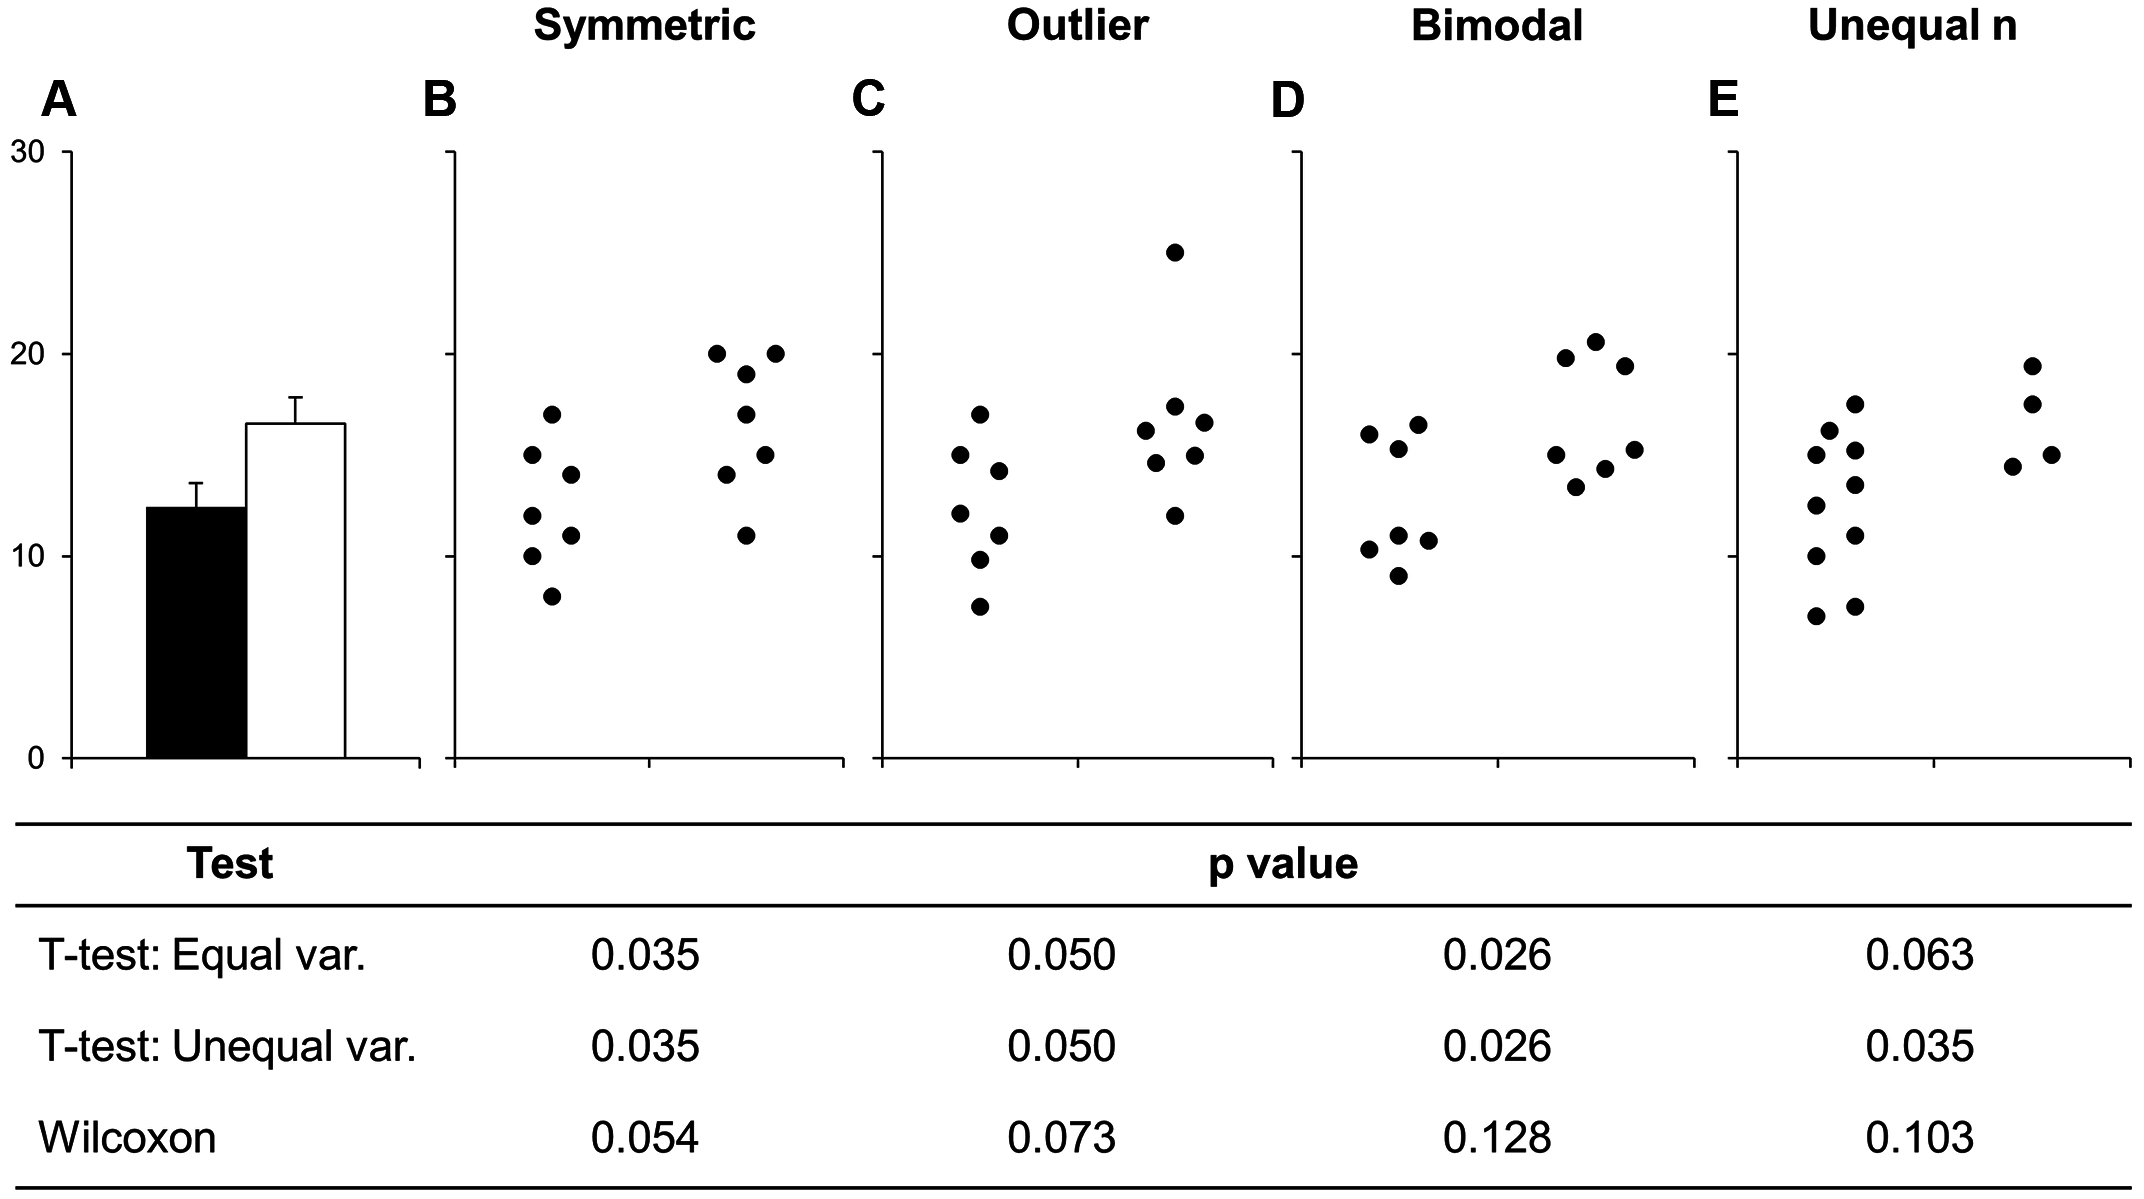
\includegraphics{fig/barplots.png}
\emph{source:} \href{http://journals.plos.org/plosbiology/article/figure/image?size=large\&id=info:doi/10.1371/journal.pbio.1002128.g001}{Weissgerber et al}

The bar chart in panel A is one that came out of all those sets of numbers in the other panels. But it really hides some important stuff, like the fact the numbers are clearly separating into two groups in panel D, or that the two samples have different sizes in panel E.

Worse than any of these is that the significant difference in the t-test is coming from just one point in panel C. From this data set you might be tempted to conclude that there is a significant difference in the two samples and if you relied on the bar chart as a visualisation then you'd never suspect there was something funny.

Some enthusiastic young science communicators have even started a Kickstarter to lobby journals to stop using, in particular, bar charts! These people, calling themselves Bar Barplots, have a nice video on one of the main problems with bar charts. Have a look at this page on Kickstarter . \href{https://www.kickstarter.com/projects/1474588473/barbarplots}{Kickstarter - Barbarplots}, especially this video \href{https://ksr-video.imgix.net/projects/2453455/video-665338-h264_high.mp4}{Kickstarter - Barbarplots video}.

Ignoring your data visualisation and just making bar plots could be an error! It's important that you spend a little time getting to know, and presenting your data as clearly and thoroughly as possible.

\hypertarget{p---one-value-to-fool-them-all}{%
\section{\texorpdfstring{\emph{p} - one value to fool them all?}{p - one value to fool them all?}}\label{p---one-value-to-fool-them-all}}

But why would you care about this, in the end a \emph{p}-value won't a \emph{p}-value help you see real differences and make this all easy? Sadly, that isn't true. Let's do an experiment to test that.

\hypertarget{ten-thousand-random-numbers}{%
\subsection{Ten Thousand Random Numbers}\label{ten-thousand-random-numbers}}

Below is a set of figures that show different views of the same set of data. Every frame of the 100 frames shows a different sampling from the same pool of 10,000 random normally distributed numbers.

\begin{figure}
\centering
\includegraphics{fig/animation.gif}
\caption{Random Sample Plots}
\end{figure}

Step-by-step, here's how these figures are made.

\begin{enumerate}
\def\labelenumi{\arabic{enumi}.}
\tightlist
\item
  Generate a pool of 10,000 random numbers (mean 5, sd 1)
\item
  From that, select 10 and call it sample 1.
\item
  Select another 10, call it sample 2.
\item
  Draw plots comparing each sample
\item
  Do an independent \emph{t}-test on the sample 1 and sample 2 to test for significant differences in means.
\end{enumerate}

The figures are plotted with a red border if \emph{p} comes up less than 0.05. The thing is, the samples are from the same background pool, so intuitively you might suspect that none should be different from the others. The reason that some of them do is because a \emph{p} value only states that the difference observed occurs by chance in \emph{p} of all events, so for 100, we'd expect 5 to be marked out by chance. In this run of the experiment we get three. Here they are:

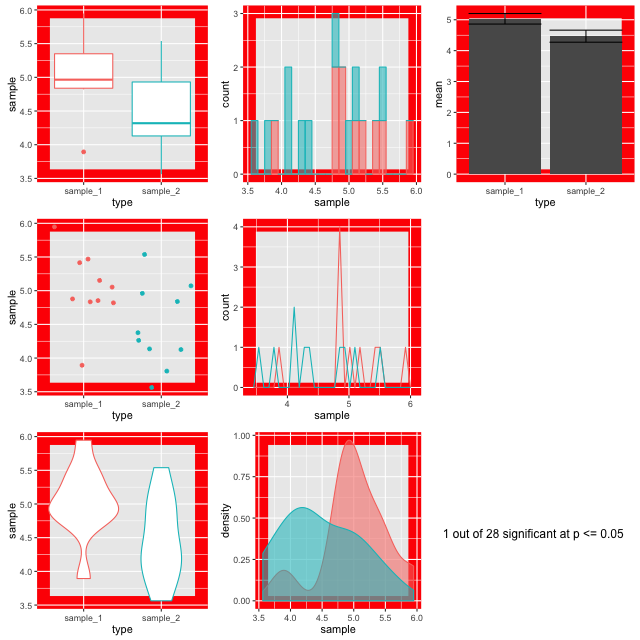
\includegraphics{fig/file_28.png}
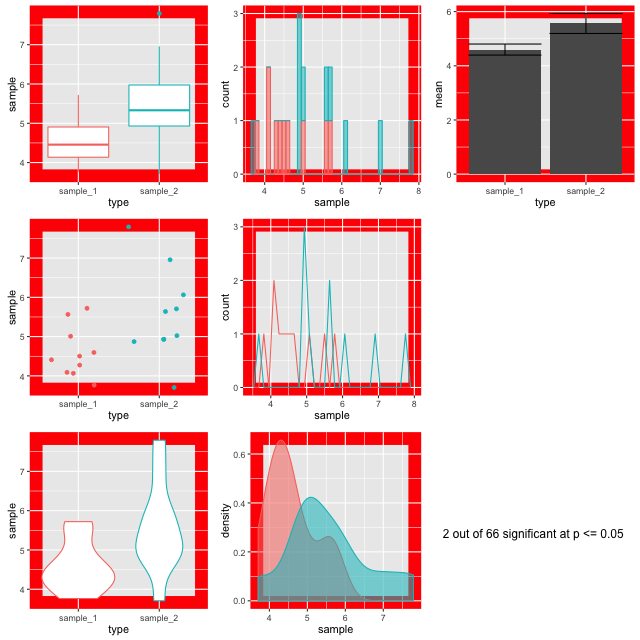
\includegraphics{fig/file_66.png}
\includegraphics{fig/file_88.png}

Look at the different plots for each. It is observable that for all these the barplots look very convincingly different. But in the context with the other plots its clear that they aren't showing the whole of the story (or in fact much of it). The boxplots (top left) do a good job of showing the range and the violin and density plots (bottom row) do a good job of showing the shape. It is only really the point plot (first column, middle row) that reveals the positions of the data points and shows that the conclusion of the \emph{p} value is likely skewed by one or two points in each sample. Concluding differences on this basis is \emph{really} unsafe.

Hence, the conclusion from this is that a range of visualisations is necessary to allow us to have confidence in our \emph{p} values and understand the shapes of our data. Drawing box plots and sticking to \emph{p} religiously is going to make us wrong more than we'd like!

\hypertarget{ggplot2-an-r-package-for-beautiful-visualisations}{%
\section{\texorpdfstring{\emph{ggplot2} An R package for beautiful visualisations}{ggplot2 An R package for beautiful visualisations}}\label{ggplot2-an-r-package-for-beautiful-visualisations}}

In this tutorial we are going to use \emph{ggplot2} a package in R to make some clear, informative, thorough visualisations that will help us with our analysis. Here's an example of the sort of thing you can get from \emph{ggplot}:

\begin{figure}
\centering
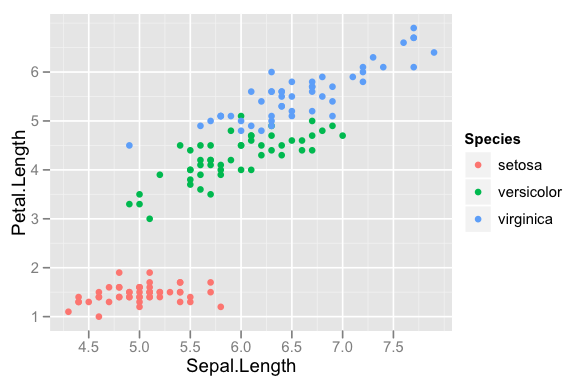
\includegraphics{fig/sepal-vs-petal-specied.png}
\caption{ggplot 2 iris data}
\end{figure}

\emph{ggplot2} is a library in the R statistical programming language - but we won't be learning to program here. The \emph{gg} part stands for `grammar of graphics', and \emph{ggplot2} is a small grammar that describes plots that should be built on top of data - effectively allowing a user to write their own plot description and have the computer work out what to do, so no programming is needed, just an appreciation of the grammar that is used to describe the plot.

\hypertarget{r-fundamentals}{%
\chapter{R Fundamentals}\label{r-fundamentals}}

\hypertarget{about-this-chapter}{%
\section{About this chapter}\label{about-this-chapter}}

\begin{enumerate}
\def\labelenumi{\arabic{enumi}.}
\tightlist
\item
  Questions:
\end{enumerate}

\begin{itemize}
\tightlist
\item
  How do I use R?
\end{itemize}

\begin{enumerate}
\def\labelenumi{\arabic{enumi}.}
\setcounter{enumi}{1}
\tightlist
\item
  Objectives:
\end{enumerate}

\begin{itemize}
\tightlist
\item
  Become familiar with R syntax
\item
  Understand the concepts of objects and assignment
\item
  Get exposed to a few functions
\end{itemize}

\begin{enumerate}
\def\labelenumi{\arabic{enumi}.}
\setcounter{enumi}{2}
\tightlist
\item
  Keypoints:
\end{enumerate}

\begin{itemize}
\tightlist
\item
  R's capabilities are provided by functions
\item
  R users call functions and get results
\end{itemize}

\hypertarget{working-with-r}{%
\section{Working with R}\label{working-with-r}}

In this workshop we'll use R in the extremely useful RStudio software. For the most part we'll work interactively, meaning we'll type stuff straight into the R console in RStudio (Usually this is a window on the left or lower left) and get our results there too (usually in the console or in a window on the right).

Panels like the ones below mimic the interaction with R and first show the thing to type into R, and below the calculated result from R.

Let's look at how R works by using it for it's most basic job - as a calculator:

\begin{Shaded}
\begin{Highlighting}[]
 \DecValTok{3} \OperatorTok{+}\StringTok{ }\DecValTok{5}
\end{Highlighting}
\end{Shaded}

\begin{verbatim}
## [1] 8
\end{verbatim}

\begin{Shaded}
\begin{Highlighting}[]
 \DecValTok{12} \OperatorTok{*}\StringTok{ }\DecValTok{2}
\end{Highlighting}
\end{Shaded}

\begin{verbatim}
## [1] 24
\end{verbatim}

\begin{Shaded}
\begin{Highlighting}[]
 \DecValTok{1} \OperatorTok{/}\StringTok{ }\DecValTok{3}
\end{Highlighting}
\end{Shaded}

\begin{verbatim}
## [1] 0.3333333
\end{verbatim}

\begin{Shaded}
\begin{Highlighting}[]
 \DecValTok{12} \OperatorTok{*}\StringTok{ }\DecValTok{2}
\end{Highlighting}
\end{Shaded}

\begin{verbatim}
## [1] 24
\end{verbatim}

Fairly straightforward, we type in the expression and we get a result. That's how this whole book will work, you type the stuff in, and get answers out. It'll be easiest to learn if you go ahead and copy the examples one by one. Try to resist the urge to use copy and paste. Typing longhand really encourages you to look at what you're entering.

As far as the R output itself goes, it's really straightforward - its just the answer with a \texttt{{[}1{]}} stuck on the front. This \texttt{{[}1{]}} tells us how many items through the output we are. Often R will return long lists of numbers and it can be helpful to have this extra information.

\hypertarget{variables}{%
\section{Variables}\label{variables}}

We can save the output of operations for later use by giving it a name using the assignment symbol \texttt{\textless{}-}. Read this symbol as `gets', so \texttt{x\ \textless{}-\ 5} reads as `x gets 5'. These names are called variables, because the value they are associated with can change.

Let's give five a name, \texttt{x} then refer to the value 5 by it's name. We can then use the name in place of the value. In the jargon of computing we say we are assigning a value to a variable.

\begin{Shaded}
\begin{Highlighting}[]
\NormalTok{ x <-}\StringTok{ }\DecValTok{5}
\NormalTok{ x}
\end{Highlighting}
\end{Shaded}

\begin{verbatim}
## [1] 5
\end{verbatim}

\begin{Shaded}
\begin{Highlighting}[]
\NormalTok{ x }\OperatorTok{*}\StringTok{ }\DecValTok{2}
\end{Highlighting}
\end{Shaded}

\begin{verbatim}
## [1] 10
\end{verbatim}

\begin{Shaded}
\begin{Highlighting}[]
\NormalTok{y <-}\StringTok{ }\DecValTok{3}
\NormalTok{x }\OperatorTok{*}\StringTok{ }\NormalTok{y}
\end{Highlighting}
\end{Shaded}

\begin{verbatim}
## [1] 15
\end{verbatim}

This is of course of limited value with just numbers but is of great value when we have large datasets, as the whole thing can be referred to by the variable.

\hypertarget{using-objects-and-functions}{%
\subsection{Using objects and functions}\label{using-objects-and-functions}}

At the top level, R is a simple language with two types of thing: functions and objects. As a user you will use functions to do stuff, and get back objects as an answer. Functions are easy to spot, they are a name followed by a pair of brackets. A function like \texttt{mean()} is the function for calculating a mean. The options (or arguments) for the function go inside the brackets:

\begin{Shaded}
\begin{Highlighting}[]
\KeywordTok{sqrt}\NormalTok{(}\DecValTok{16}\NormalTok{)}
\end{Highlighting}
\end{Shaded}

\begin{verbatim}
## [1] 4
\end{verbatim}

Often the result from a function will be more complicated than a simple number object, often it will be a vector (simple list), like from the \texttt{rnorm()} function that returns lists of random numbers

\begin{Shaded}
\begin{Highlighting}[]
\KeywordTok{rnorm}\NormalTok{(}\DecValTok{100}\NormalTok{)}
\end{Highlighting}
\end{Shaded}

\begin{verbatim}
##   [1] -1.87348951  0.22366083  1.04537876  1.18642540 -1.00097271  0.71392923
##   [7]  0.39131001  1.36073433 -1.06406960  0.12798245  0.06224181 -1.34481036
##  [13]  0.08294133  0.16901502  0.47127447 -1.83443792 -0.30507286 -0.95109207
##  [19] -2.30659527  1.17444366  0.07753248  1.89622737 -1.49546907 -0.35016241
##  [25] -2.01667631  1.31452109 -0.85422757 -2.06736300 -0.81983173 -1.33634072
##  [31]  1.45247233  1.09458002  1.18454056  0.41945299 -0.13367727  0.24543311
##  [37] -0.42486462  1.48068266  0.48421069  0.81762383  0.18761798  0.60618714
##  [43]  0.72651222  1.26144777 -0.17387570  0.33861155  0.71844700 -1.13175451
##  [49] -0.45727074  0.32069733  0.42558649  0.16464947 -1.32784233 -0.08478824
##  [55]  0.91609945  1.31949308  0.74152844 -0.72382332 -0.31620121 -0.62017300
##  [61] -0.26876702 -0.52292215 -0.59233868  2.11431858 -0.97621933 -1.77373056
##  [67] -1.86838446  0.75842429 -0.33387079 -0.48985552  1.48674339 -1.68439580
##  [73] -0.14568001  1.61909301  0.02216918 -1.67241780 -2.02229780  0.20750723
##  [79]  1.33216027  0.26101861 -0.61169470  0.30393901  0.42784336  0.35010079
##  [85]  0.64907856  0.99545135  0.01993294  0.48012765 -0.31189773  0.87142918
##  [91] -1.16257040  0.07339797 -2.32344449 -0.14456522  0.69117043  0.19954687
##  [97]  0.88521508 -0.10784865  0.63535808  1.43216256
\end{verbatim}

We can combine objects, variables and functions to do more complex stuff in R, here's how we get the mean of 100 random numbers.

\begin{Shaded}
\begin{Highlighting}[]
\NormalTok{numbers <-}\StringTok{ }\KeywordTok{rnorm}\NormalTok{(}\DecValTok{100}\NormalTok{)}
\KeywordTok{mean}\NormalTok{(numbers)}
\end{Highlighting}
\end{Shaded}

\begin{verbatim}
## [1] 0.1323635
\end{verbatim}

Here we created a vector object with \texttt{rnorm(100)} and assigned it to the variable \texttt{numbers}. We than used the \texttt{mean()} function, passing it the variable \texttt{numbers}. The \texttt{mean()} function returned the mean of the hundred random numbers.

\hypertarget{dataframes}{%
\section{Dataframes}\label{dataframes}}

One of the more common objects that R uses is a dataframe. The dataframe is a rectangular table-like object that contains data, think of it like a spreadsheet tab. Like the spreadsheet, the dataframe has rows and columns, the columns have names and the different columns can have different types of data in. Here's a little one

\begin{verbatim}
##   names age    score
## 1 Guido  24 10.92035
## 2 Marty  45 27.41630
## 3  Alan  11 19.41638
\end{verbatim}

Usually we get a dataframe by loading in data from an external source or as a result from functions, occasionally we'll want to hand make one, which can be done with various functions, \texttt{data.frame} being the most common.

\begin{Shaded}
\begin{Highlighting}[]
\KeywordTok{data.frame}\NormalTok{(}
  \DataTypeTok{names =} \KeywordTok{c}\NormalTok{(}\StringTok{"Guido"}\NormalTok{, }\StringTok{"Marty"}\NormalTok{, }\StringTok{"Alan"}\NormalTok{),}
  \DataTypeTok{age =} \KeywordTok{c}\NormalTok{(}\DecValTok{24}\NormalTok{,}\DecValTok{45}\NormalTok{,}\DecValTok{11}\NormalTok{),}
  \DataTypeTok{score =} \KeywordTok{runif}\NormalTok{(}\DecValTok{3}\NormalTok{) }\OperatorTok{*}\StringTok{ }\DecValTok{100}
\NormalTok{)}
\end{Highlighting}
\end{Shaded}

\hypertarget{packages}{%
\section{Packages}\label{packages}}

Many of the tools we use in will come in R packages, little nuggets of code that group related functions together. Installing new packages can be done using the \texttt{Packages} pane of RStudio or the \texttt{install.packages()} function. When we wish to use that code we use the \texttt{library()} function

\begin{Shaded}
\begin{Highlighting}[]
\KeywordTok{library}\NormalTok{(somepackage)}
\end{Highlighting}
\end{Shaded}

\hypertarget{using-r-help}{%
\section{Using R Help}\label{using-r-help}}

R provides a command, called \texttt{?} that will display the documentation for functions. For example \texttt{?mean} will display the help for the \texttt{mean()} function.

\begin{Shaded}
\begin{Highlighting}[]
\NormalTok{?mean}
\end{Highlighting}
\end{Shaded}

As in all programming languages the internal documentation in R is written with some assumption that the reader is familiar with the language. This can be a pain when you are starting out as the help will seem a bit obscure at times. Don't worry about this, usually the \texttt{Examples} section will give you a good idea of how to use the function and as your experience grows then the more things will make more sense.

\begin{roundup}
\begin{itemize}
\tightlist
\item
  R is an excellent and powerful statistical computing environment
\end{itemize}
\end{roundup}

\begin{task}
Complete the interactive tutorial online \url{https://danmaclean.shinyapps.io/r-start}
\end{task}

  \bibliography{book.bib,packages.bib}

\end{document}
